\documentclass{standalone}

\usepackage{tikz}

\begin{document}
\Large
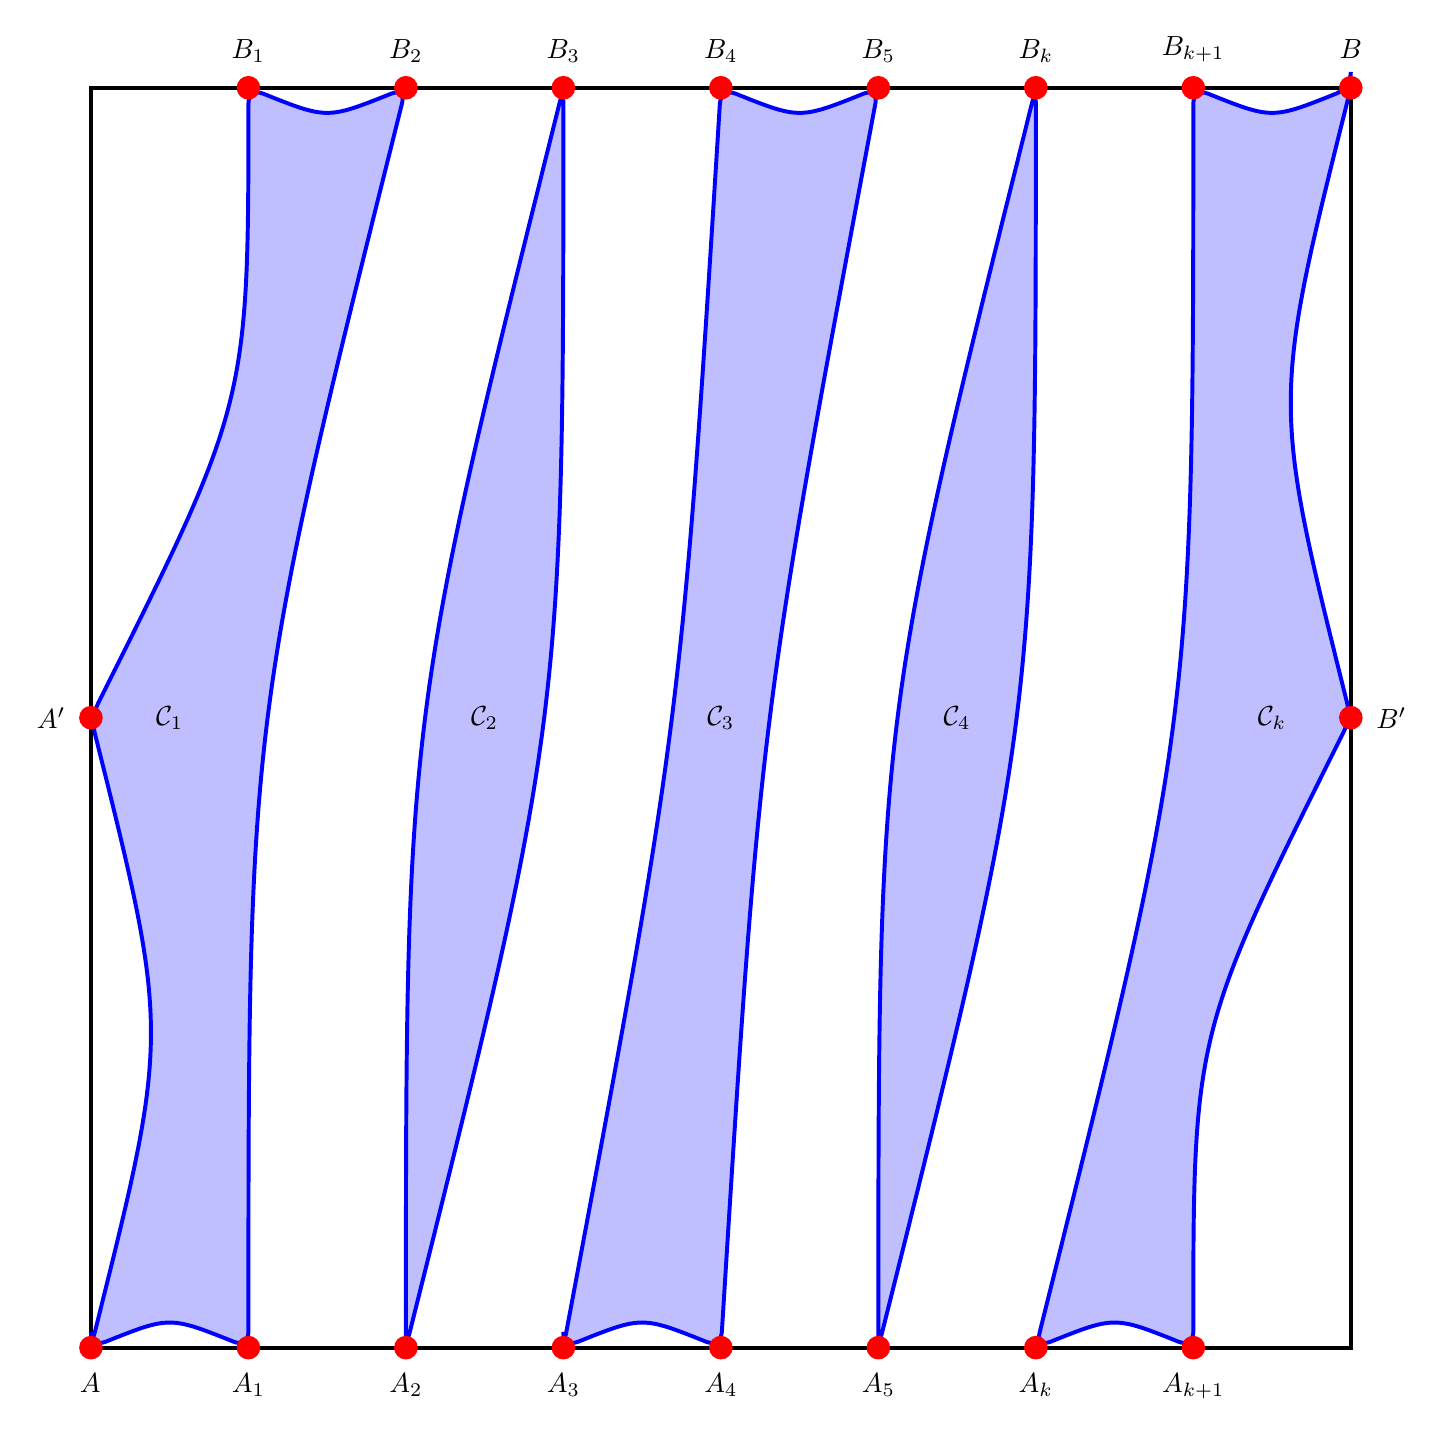
\begin{tikzpicture}
% \draw[help lines, black!30] (0,0) grid (12,12);
\draw[line width=0.5mm, black] 
    (0,0) rectangle (16,16);
\draw[line width=0.5mm, blue, fill=blue!25, rounded corners=2mm] 
    (0,0) ..controls+(1,0.4).. 
    (2,0) ..controls+(0,8).. 
    (4,16) ..controls+(-1,-0.4).. 
    (2,16) ..controls+(0,-4).. 
    (0,8) ..controls+(1,-4).. cycle % 1
    (4,0) ..controls+(2,8).. 
    (6,16) ..controls+(-2,-8).. cycle %2
    (6,0) ..controls+(1,0.4).. 
    (8,0) ..controls+(0.5,8)..
    (10,16) ..controls+(-1,-0.4).. 
    (8,16) ..controls+(-0.5,-8).. cycle %3
    (10,0) ..controls+(2,8).. 
    (12,16) ..controls+(-2,-8).. cycle %4
    (16,16) ..controls+(-1,-0.4).. 
    (14,16) ..controls+(0,-8).. 
    (12,0) ..controls+(1,0.4).. 
    (14,0) ..controls+(0,4).. 
    (16,8) ..controls+(-1,4).. cycle; %5
\fill[red] foreach \a in 
    {(0,0), (2,0), (4,0), (6,0), (8,0), (10,0), (12,0), (14,0), (0,8),
     (2,16), (4,16), (6,16), (8,16), (10,16), (12,16), (14,16), (16,16), (16,8)}
    {\a circle (1.5mm)};
\foreach \a/\b in 
    {(0,0)/, (2,0)/1, (4,0)/2, (6,0)/3, (8,0)/4, (10,0)/5, (12,0)/k, (14,0)/k+1}
    {\node[below=2mm] at \a {$A_{\b}$};};
\foreach \a/\b in 
    {(2,16)/1, (4,16)/2, (6,16)/3, (8,16)/4, (10,16)/5, (12,16)/k, (14,16)/k+1, (16,16)/}
    {\node[above=2mm] at \a {$B_{\b}$};};
\node[left=2mm] at (0,8) {$A'$};
\node[right=2mm] at (16,8) {$B'$};
\foreach \a/\b in 
    {(1,8)/1, (5,8)/2, (8,8)/3, (11,8)/4, (15,8)/k}
    {\node at \a {$\mathcal{C}_{\b}$};};


\end{tikzpicture}
\end{document}